\begin{figure}[h]
\centering
\small
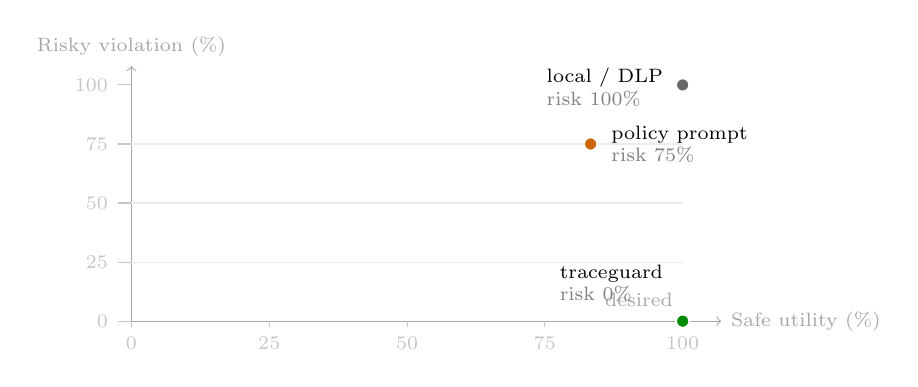
\begin{tikzpicture}[x=7.0cm,y=3.0cm,every node/.style={font=\scriptsize}]
  \draw[->, gray!70] (0,0) -- (1.07,0) node[right] {Safe utility (\%)};
  \draw[->, gray!70] (0,0) -- (0,1.08) node[above] {Risky violation (\%)};
  \draw[gray!45] (0.00,0) -- (0.00,-0.025) node[below] {0};
  \draw[gray!45] (0,0.00) -- (-0.025,0.00) node[left] {0};
  \draw[gray!45] (0.25,0) -- (0.25,-0.025) node[below] {25};
  \draw[gray!45] (0,0.25) -- (-0.025,0.25) node[left] {25};
  \draw[gray!15] (0,0.25) -- (1,0.25);
  \draw[gray!45] (0.50,0) -- (0.50,-0.025) node[below] {50};
  \draw[gray!45] (0,0.50) -- (-0.025,0.50) node[left] {50};
  \draw[gray!15] (0,0.50) -- (1,0.50);
  \draw[gray!45] (0.75,0) -- (0.75,-0.025) node[below] {75};
  \draw[gray!45] (0,0.75) -- (-0.025,0.75) node[left] {75};
  \draw[gray!15] (0,0.75) -- (1,0.75);
  \draw[gray!45] (1.00,0) -- (1.00,-0.025) node[below] {100};
  \draw[gray!45] (0,1.00) -- (-0.025,1.00) node[left] {100};
  \node[anchor=south east, text=gray!70] at (1,0.02) {desired};
  \filldraw[black!35, draw=white, line width=0.7pt] (1.000,1.000) circle (2.4pt);
  \filldraw[black!60, draw=white, line width=0.7pt] (1.000,1.000) circle (2.4pt);
  \node[anchor=east, align=left] at (0.982,0.990) {local / DLP\\{\color{gray}risk 100\%}};
  \filldraw[orange!80!black, draw=white, line width=0.7pt] (0.833,0.750) circle (2.4pt);
  \node[anchor=west, align=left] at (0.853,0.750) {policy prompt\\{\color{gray}risk 75\%}};
  \filldraw[green!55!black, draw=white, line width=0.7pt] (1.000,0.000) circle (2.4pt);
  \node[anchor=south east, align=left] at (0.982,0.040) {traceguard\\{\color{gray}risk 0\%}};
\end{tikzpicture}
\caption{Security-utility frontier on the 24-task \texttt{gpt-4.1-mini} API subset. The desired region is high safe-control utility and low risky-violation rate. Local guards and DLP preserve utility but violate every risky task; TraceGuard preserves utility while eliminating risky violations.}
\label{fig:api-security-utility}
\end{figure}
